\documentclass{beamer}
\usepackage{amsmath}
\usepackage{amssymb}
\usepackage{bbm}
\usepackage{pgf}
\usepackage{tikz}
\usepackage{nicefrac}
\usetikzlibrary{matrix}
\usetheme{boxes}
\newcommand{\fig}{figures} % common figure path
\newcommand{\frnzplt}{FranzPlot }
\newcommand{\dbbslsh}{\textbackslash \textbackslash} % common figure path
\newcommand{\norm}[1]{\left\lVert#1\right\rVert}
\newcommand{\parallelsum}{\mathbin{\!/\mkern-5mu/\!}}
\DeclareMathSymbol{\shortminus}{\mathbin}{AMSa}{"39}


\title[Curve e Sup. - Lab 3]{Curve e Superfici per il Design \\ Laboratorio - 3}
\author[Prof. Parolini]{Prof. Nicola Parolini}
%\institute[dimat]{Long Inst.}
\date{31 Ottobre 2019}

\begin{document}
\begin{frame}
\maketitle
\end{frame}

\begin{frame}
\frametitle{Materiali}
Il materiale per l'esercitazione di oggi:
\begin{itemize}
\item Questa presentazione \\ (\texttt{Materiale Didattico/Laboratori/lab 3/lab3\_testo.pdf});
%\item Il file \texttt{es\_dado\_ref.toml} con l'esercizio risolto della passata esercitazione.
\item L'eseguibile del \frnzplt \\ (\texttt{Software/Franzplot 19.08 - Windows.exe})
\end{itemize}
\end{frame}

\begin{frame}
\frametitle{Rotazioni: Asse x}
\begin{equation}
R_x(\theta) = 
\begin{bmatrix}
1 & 0 & 0 \\
0 & \mbox{cos}(\theta) & - \mbox{sen}(\theta)\\
0 & \mbox{sen}(\theta) & \mbox{cos}(\theta)
\end{bmatrix}
\end{equation}
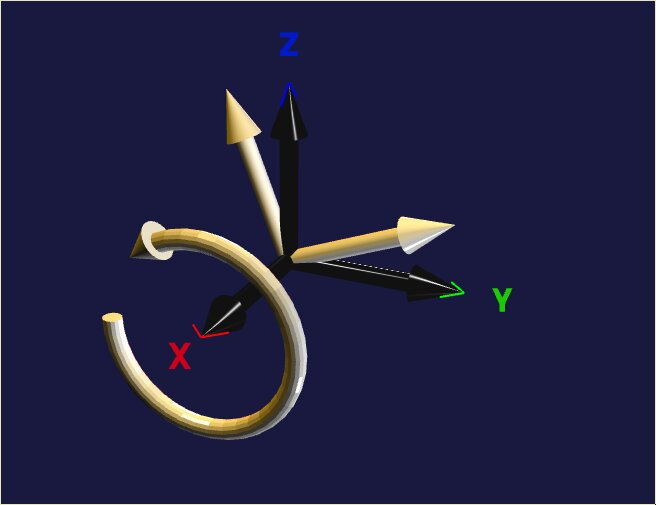
\includegraphics[width=0.6\textwidth]{\fig/rot_x.jpeg}
\end{frame}
\begin{frame}
\frametitle{Rotazioni: Asse y}
\begin{equation}
R_y(\theta) = 
\begin{bmatrix}
\mbox{cos}(\theta) & 0 & \mbox{sen}(\theta)\\
0 & 1 & 0 \\
-\mbox{sen}(\theta)& 0 & \mbox{cos}(\theta)
\end{bmatrix}
\end{equation}
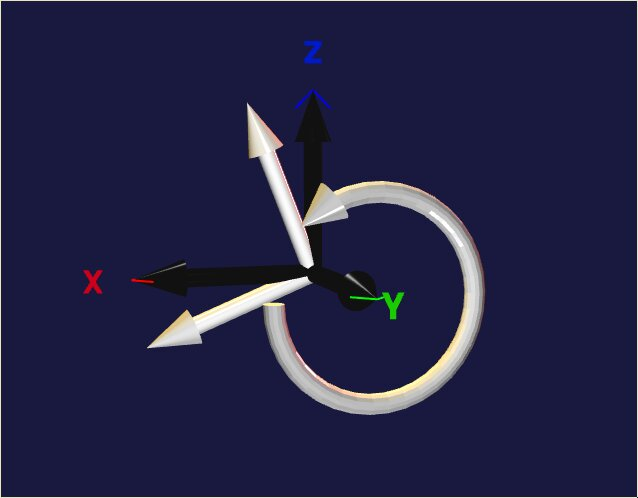
\includegraphics[width=0.6\textwidth]{\fig/rot_y.jpeg}
\end{frame}
\begin{frame}
\frametitle{Rotazioni: Asse z}
\begin{equation}
R_z(\theta) = 
\begin{bmatrix}
\mbox{cos}(\theta) & - \mbox{sen}(\theta) & 0\\
\mbox{sen}(\theta) & \mbox{cos}(\theta)   & 0\\ 
0 & 0 & 1 
\end{bmatrix}
\end{equation}
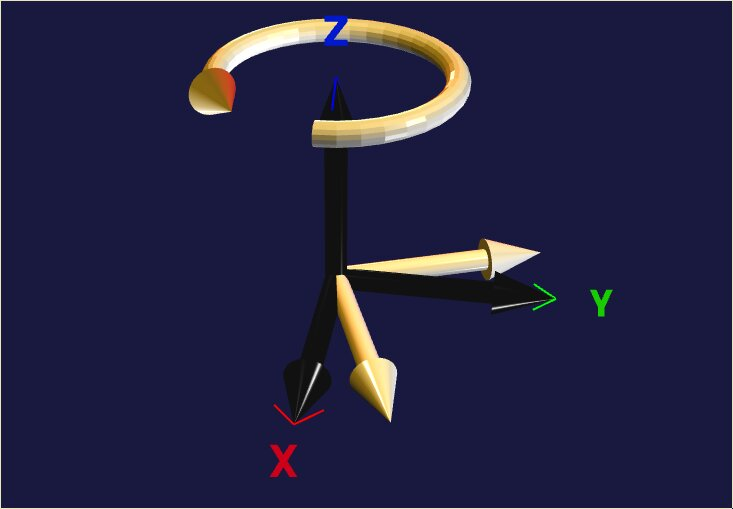
\includegraphics[width=0.6\textwidth]{\fig/rot_z.jpeg}
\end{frame}
%
\begin{frame}
\frametitle{Tagli}
\begin{columns}
\begin{column}{0.48\textwidth}
Taglio in direzione x sulle facce con normale y:
\begin{equation}
T_{xy}=\begin{bmatrix}
    1 & k_x & 0\\
    0 & 1   & 0\\
    0 & 0   & 1
    \end{bmatrix}
\end{equation}
\end{column}
\begin{column}{0.48\textwidth}
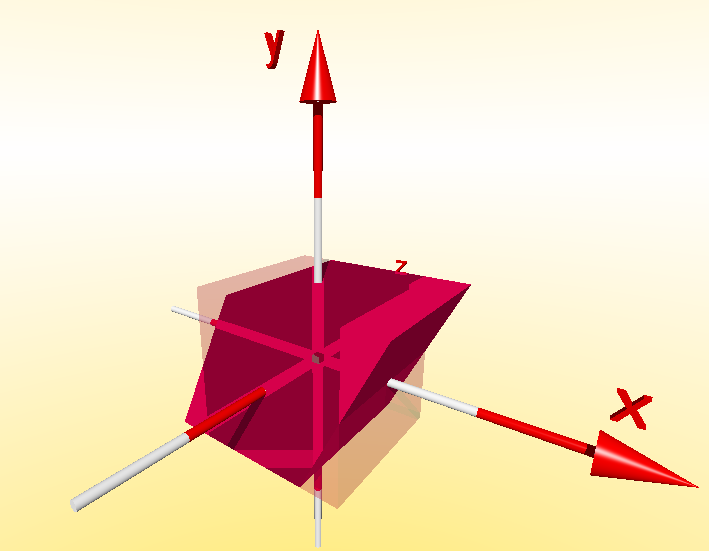
\includegraphics[width=0.8\textwidth]{\fig/cut_tx.png}
\end{column}
\end{columns}
%
\begin{columns}
\begin{column}{0.48\textwidth}
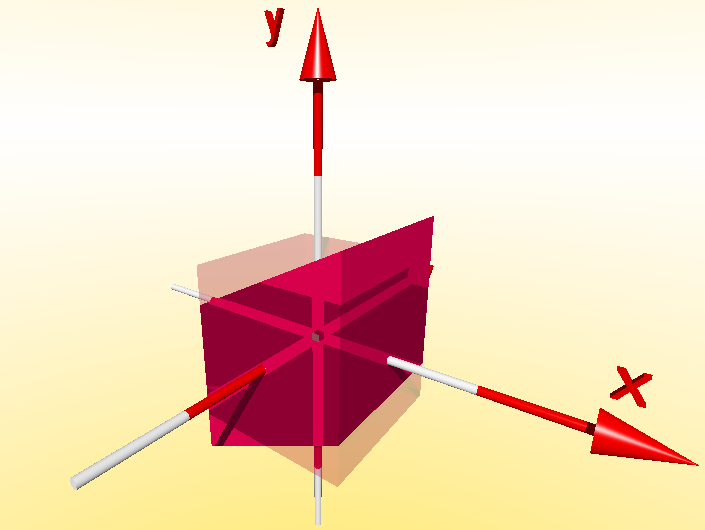
\includegraphics[width=0.8\textwidth]{\fig/cut_ty.png}
\end{column}
\begin{column}{0.48\textwidth}
Taglio in direzione y sulle facce con normale x:
\begin{equation}
T_{yx}=\begin{bmatrix}
    1   & 0 & 0\\
    k_y & 1 & 0\\
    0   & 0 & 1
    \end{bmatrix}
\end{equation}
\end{column}
\end{columns}
\end{frame}
%
\begin{frame}
\frametitle{Tagli[2]}
\begin{columns}
\begin{column}{0.48\textwidth}
Taglio in direzione z sulle facce con normale x:
\begin{equation}
T_{zx}=\begin{bmatrix}
    1 & 0 & 0\\
    0 & 1 & 0\\
    k_z & 0 & 1
    \end{bmatrix}
\end{equation}
\end{column}
\begin{column}{0.48\textwidth}
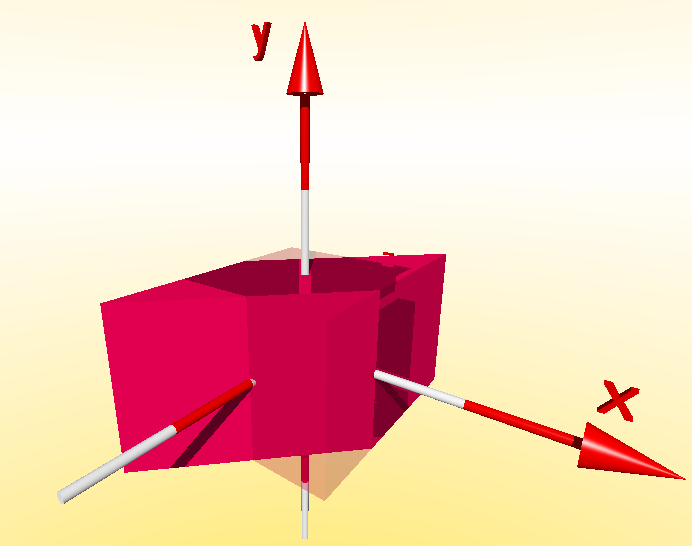
\includegraphics[width=0.8\textwidth]{\fig/cut_tz-x.png}
\end{column}
\end{columns}
%
%\begin{block}{}
\begin{columns}
\begin{column}{0.48\textwidth}
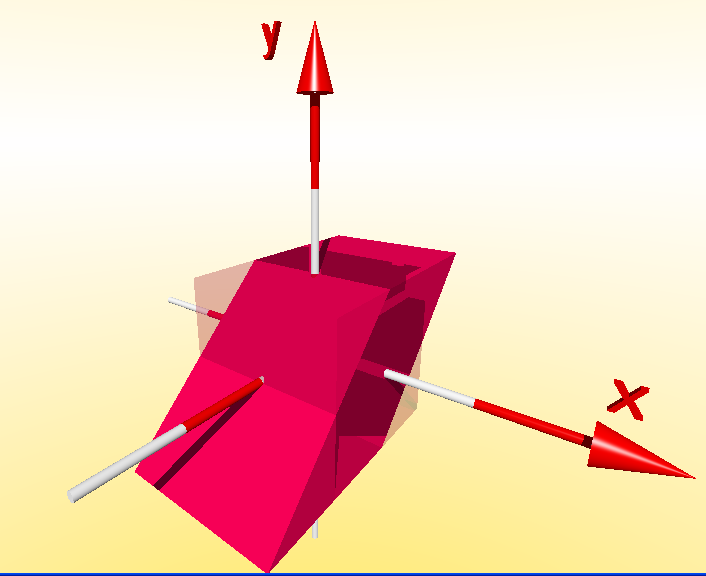
\includegraphics[width=0.8\textwidth]{\fig/cut_tz-y.png}
\end{column}
\begin{column}{0.48\textwidth}
Taglio in direzione z sulle facce con normale y:
\begin{equation}
T_{zy}=\begin{bmatrix}
    1 & 0 & 0\\
    0 & 1 & 0\\
    0 & k_z & 1
    \end{bmatrix}
\end{equation}
\end{column}
\end{columns}
%\end{block}
\end{frame}
%
\begin{frame}
\frametitle{Scalatura, Riflessione,Proiezione}
\begin{itemize}
\item Scalatura
\begin{equation}
S = \begin{bmatrix}
    S_x & 0 & 0\\
    0 & S_y & 0\\
    0 & 0 & S_z
    \end{bmatrix}
\end{equation}
\item Riflessione
\begin{equation}
F = \begin{bmatrix}
      1 & 0 & 0\\
      0 & 1 & 0\\
      0 & 0 & 1
    \end{bmatrix}
    -2~\begin{bmatrix}
    n_x \\
    n_y \\
    n_z
    \end{bmatrix} 
    ~\begin{bmatrix}
    n_x & n_y & n_z
    \end{bmatrix}
\end{equation}
\item Proiezione
\begin{equation}
 P = \begin{bmatrix}
      1 & 0 & 0\\
      0 & 1 & 0\\
      0 & 0 & 1
    \end{bmatrix}
    -\begin{bmatrix}
    n_x \\
    n_y \\
    n_z
    \end{bmatrix} 
    ~\begin{bmatrix}
    n_x & n_y & n_z
    \end{bmatrix}
\end{equation}
\end{itemize}
\end{frame}
%
\begin{frame}
\frametitle{Coordinate omogenee}
\begin{displaymath}
\begin{bmatrix}
a_{11} & a_{12} & a_{13} & t_1 \\
a_{21} & a_{22} & a_{23} & t_2 \\
a_{31} & a_{32} & a_{33} & t_3 \\
0      &    0   &  0     & 1 
\end{bmatrix}
~\begin{bmatrix}
x \\ y\\ z\\ 1
\end{bmatrix}
=  
\begin{bmatrix}
a_{11}x + a_{12}y + a_{13}z + t_1 \\
a_{21}x + a_{22}y + a_{23}z + t_2 \\
a_{31}x + a_{32}y + a_{33}z + t_3 \\
 1
\end{bmatrix}
\end{displaymath}
\end{frame}



\section{Esercizi}
%
\begin{frame}
\frametitle{Esercizio 1 - Moltiplicazioni matrice-matrice}
Date le due matrici:
\begin{displaymath}
    A =
\begin{bmatrix}
   1 &  2 &  0 &  0 \\
  -2 &  1 &  0 &  1 \\
   3 &  0 &  1 & -1 \\
   0 &  0 &  0 &  1
\end{bmatrix}
\qquad
B = 
\begin{bmatrix}
   1 &  0 &  3 &  1 \\
   2 &  1 &  0 &  1 \\
   2 &  0 & -3 &  0 \\
   0 &  0 &  0 &  1 
\end{bmatrix}
\end{displaymath}
\begin{itemize}
\item Calcolare la matrice $M = A B$
\item Calcolare la matrice $N = B A$
\end{itemize}
\end{frame}
%
\begin{frame}
\frametitle{Esercizio 1 - i}
Calcolo di M:
\begin{displaymath}
    M =
\begin{bmatrix}
   1 &  2 &  0 &  0 \\
  -2 &  1 &  0 &  1 \\
   3 &  0 &  1 & -1 \\
   0 &  0 &  0 &  1
\end{bmatrix}
\begin{bmatrix}
   1 &  0 &  3 &  1 \\
   2 &  1 &  0 &  1 \\
   2 &  0 & -3 &  0 \\
   0 &  0 &  0 &  1 
\end{bmatrix}
\end{displaymath}

La matrice M risultante sar\`a una matrice $4\times4$, e dobbiamo calcolarla elemento per elemento:

\begin{displaymath}
    M =
\begin{bmatrix}
    m_{11} & m_{12} & m_{13} & m_{14} \\
    m_{21} & m_{22} & m_{23} & m_{24} \\
    m_{31} & m_{32} & m_{33} & m_{34} \\
    m_{41} & m_{42} & m_{43} & m_{44}
\end{bmatrix}
\end{displaymath}

\end{frame}

\begin{frame}
\frametitle{Esercizio 1 - ii}

    L'elemento $m_{ij}$, ovvero quel numero contenuto nella matrice M e posizionato nella \textbf{riga i} e nella
    \textbf{colonna j}, \`e il \textbf{prodotto scalare} dei vettori \textbf{riga i-esima di A} e \textbf{colonna j-esima di B}


Vediamo il calcolo di alcuni elementi di matrice:
\begin{displaymath}
    m_{11} =
\begin{bmatrix}
    1 &  2 &  0 &  0
\end{bmatrix}
\cdot
\begin{bmatrix}
    1 \\  2 \\ 2 \\ 0
\end{bmatrix}
 = 1 \cdot 1 + 2 \cdot 2 + 0 \cdot 2 + 0 \cdot 0
 = 5
\end{displaymath}

\end{frame}

\begin{frame}
\frametitle{Esercizio 1 - iii}

\begin{displaymath}
    m_{21} =
\begin{bmatrix}
    -2 & 1 &  0 &  1
\end{bmatrix}
\cdot
\begin{bmatrix}
    1 \\  2 \\ 2 \\ 0
\end{bmatrix}
 = \shortminus 2 \cdot 1 + 1 \cdot 2 + 0 \cdot 2 + 1 \cdot 0
 = 0
\end{displaymath}


\begin{displaymath}
    m_{23} =
\begin{bmatrix}
    -2 & 1 &  0 &  1
\end{bmatrix}
\cdot
\begin{bmatrix}
    3 \\  0 \\ -3 \\ 0
\end{bmatrix}
 = \shortminus 2 \cdot 3 + 1 \cdot 0 + 0 \cdot \shortminus 3 + 1 \cdot 0
 = \shortminus 6
\end{displaymath}

E cos\`i via per tutti gli altri elementi.
\end{frame}

\begin{frame}
\frametitle{Esercizio 1 - iv}

Poich\'e ogni singolo elemento di matrice richiede il calcolo di un prodotto scalare di due vettori,
    per calcolare la matrice $M$ dovremo calcolare $\mathbf{16}$ prodotti scalari.
    \begin{itemize}
        \item Allenarsi nel calcolo a mente dei prodotti scalari ci permette di non 
            consumare quantit\`a industriali di carta.
    \end{itemize}
    Nei nostri esercizi in genere le matrici contengono molti zeri, questo semplifica molto i calcoli.
    \begin{itemize}
        \item In particolare, quando lavoriamo in coordinate omogenee \textbf{l'ultima riga} di una
            qualsiasi matrice di trasformazione \`e sempre 
$\begin{bmatrix} 0 & 0 &  0 &  1 \end{bmatrix}  $
    \end{itemize}

\end{frame}

\begin{frame}
\frametitle{Esercizio 1 - v}
Svolgendo tutti i calcoli, giungiamo al risultato:
\begin{displaymath}
    M =
\begin{bmatrix}
   5 &  2 &  3 &  3 \\
   0 &  1 & -6 &  0 \\
   5 &  0 &  6 &  2 \\
   0 &  0 &  0 &  1
\end{bmatrix}
\end{displaymath}

Per il calcolo di N, cambia l'ordine delle matrici da moltiplicare!
\begin{displaymath}
    N = B A =
\begin{bmatrix}
   1 &  0 &  3 &  1 \\
   2 &  1 &  0 &  1 \\
   2 &  0 & -3 &  0 \\
   0 &  0 &  0 &  1 
\end{bmatrix}
\begin{bmatrix}
   1 &  2 &  0 &  0 \\
  -2 &  1 &  0 &  1 \\
   3 &  0 &  1 & -1 \\
   0 &  0 &  0 &  1
\end{bmatrix}
\end{displaymath}

\end{frame}
%
\begin{frame}
\frametitle{Esercizio 1 - vi}
Poich\'e in generale la moltiplicazione tra matrici non \`e commutativa, cambia anche il risultato:
\begin{displaymath}
    N =
\begin{bmatrix}
  10 &  2 &  3 & -2 \\
   0 &  5 &  0 &  2 \\
  -7 &  4 & -3 &  3 \\
   0 &  0 &  0 &  1
\end{bmatrix}
\end{displaymath}

In generale \`e sempre necessario calcolare il risultato di un prodotto matrice-matrice
quando cerchiamo di comporre due trasformazioni! Tuttavia esiste una eccezione che vedremo pi\`u avanti.

\end{frame}
%
\begin{frame}
\frametitle{Esercizio 2}
\begin{itemize}
    \item Scrivere la matrice $S$ che descrive la scalatura con \\ $S_x = 0.5$, $S_y = 0.5$, $S_z = 1$.
    \item Scrivere la matrice $R$ che descrive la rotazione di $90^\circ$ intorno l'asse Y.
    \item Calcolare la matrice $M = R S$.
    \item Usando il \frnzplt, creare una primitiva `cono' e applicare la trasformazione rappresentata dalla matrice $M$.
    \item Verificare che la trasformazione $M$ corrisponde all'applicare \textbf{prima} una scalatura e \textbf{poi} una rotazione.
    \item Cosa succederebbe se invece applicassimo prima la rotazione e poi la scalatura? 
\end{itemize}
\end{frame}

\begin{frame}
\frametitle{Esercizio 2 - i}
Matrice di scalatura S:
\begin{displaymath}
S = 
\begin{bmatrix}
    0.5 & 0   & 0   & 0 \\
      0 & 0.5 & 0   & 0 \\
      0 & 0   & 1   & 0 \\
      0 & 0   & 0   & 1 
\end{bmatrix}
\end{displaymath}

Matrice di rotazione R:
\begin{displaymath}
R = 
\begin{bmatrix}
    \mbox{cos}(\nicefrac{\pi}{2}) & 0 & \mbox{sin}(\nicefrac{\pi}{2}) & 0\\
        0 & 1 & 0 & 0 \\
        \shortminus \mbox{sin}(\nicefrac{\pi}{2}) & 0 & \mbox{cos}(\nicefrac{\pi}{2}) & 0 \\
    0 & 0 & 0 & 1 
\end{bmatrix}
=
\begin{bmatrix}
        0 & 0 & 1 & 0\\
        0 & 1 & 0 & 0 \\
        \shortminus 1 & 0 & 0 & 0 \\
    0 & 0 & 0 & 1 
\end{bmatrix}
\end{displaymath}
\end{frame}

\begin{frame}
\frametitle{Esercizio 2 - ii}
Matrice M:
\begin{displaymath}
M = 
\begin{bmatrix}
        0 & 0 & 1 & 0\\
        0 & 1 & 0 & 0 \\
        \shortminus 1 & 0 & 0 & 0 \\
        0 & 0 & 0 & 1 
\end{bmatrix}
\begin{bmatrix}
    0.5 & 0   & 0   & 0 \\
      0 & 0.5 & 0   & 0 \\
      0 & 0   & 1   & 0 \\
      0 & 0   & 0   & 1 
\end{bmatrix}
 = 
\begin{bmatrix}
        0 & 0 & 1 & 0\\
        0 & 0.5 & 0 & 0 \\
        \shortminus 0.5 & 0 & 0 & 0 \\
        0 & 0 & 0 & 1 
\end{bmatrix}
\end{displaymath}
\end{frame}

\begin{frame}
\frametitle{Esercizio 2 - iii}
\begin{center}
\begin{tikzpicture}
\node(img1){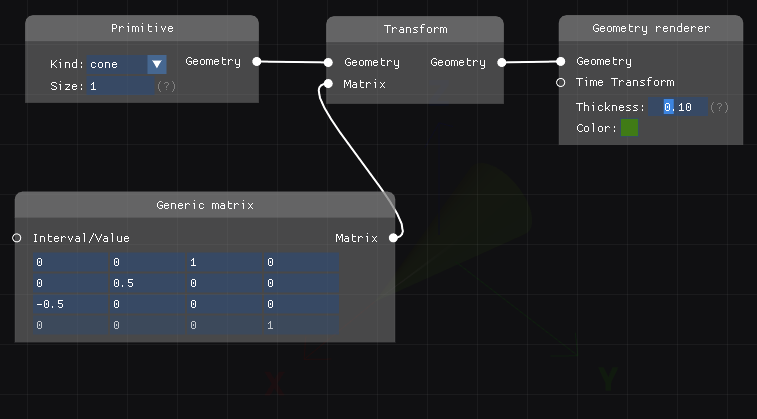
\includegraphics[width=0.8\textwidth]{\fig/lab3_es2_M.png}};
\node(img2) at (img1.south east){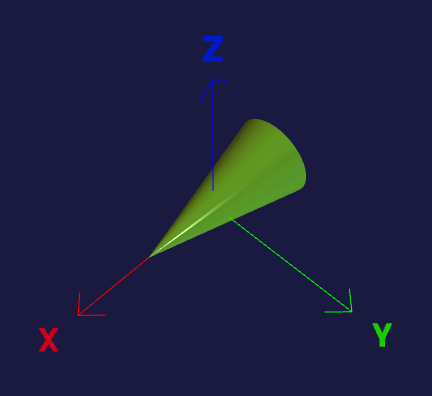
\includegraphics[width=0.4\textwidth]{\fig/lab3_es2_result.png}};
\end{tikzpicture}
\end{center}
\end{frame}

\begin{frame}
\frametitle{Esercizio 2 - iv}
Nel caso in cui si inverta l'ordine delle trasformazioni il risultato \`e sensibilmente diverso.
Il grafo diventa il seguente:
    \vspace{0.25cm}
\begin{center}
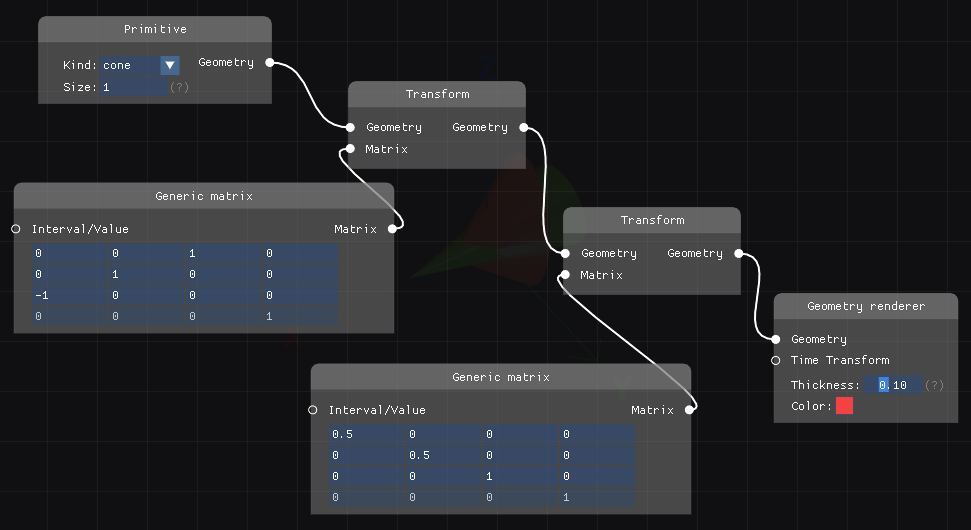
\includegraphics[width=0.9\textwidth]{\fig/lab3_es2_othergraph.png}
\end{center}

\end{frame}

\begin{frame}
\frametitle{Esercizio 2 - v}
E queste sono due viste del confronto tra il cono al punto precedente e quello ottenuto ora.
\begin{center}
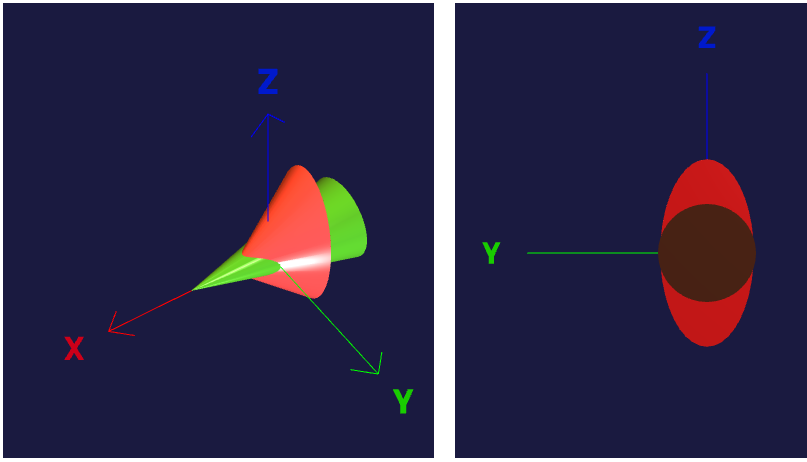
\includegraphics[width=0.8\textwidth]{\fig/lab3_es2_comparison.png}
\end{center}

Notiamo che la base \`e diventata una ellisse, perch\'e il cerchio stavolta \`e stato riscalato soltanto lungo l'asse Y.
    L'altezza, che prima non veniva modificata, ora \`e stata dimezzata.
\end{frame}

%\begin{frame}
%Il grafo che descrive la scena:
%    \vspace{0.5cm}
%\begin{center}
%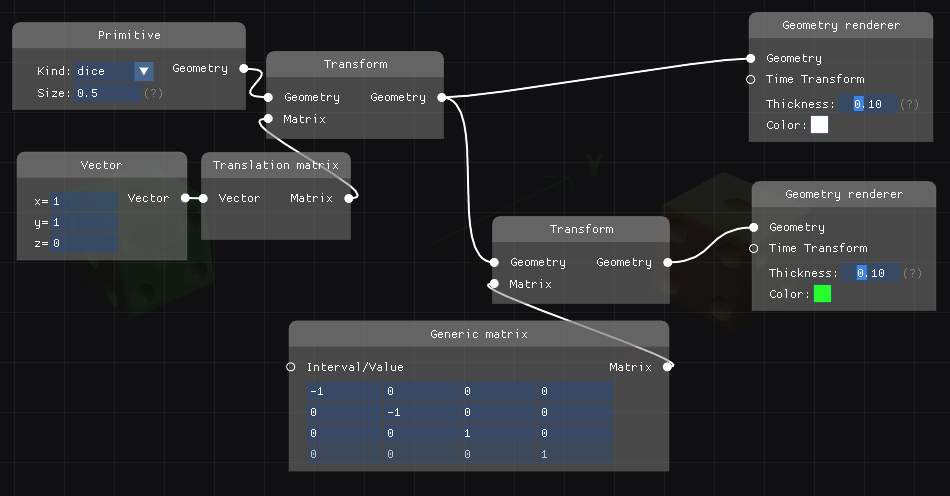
\includegraphics[width=\textwidth]{\fig/lab2_es1_a.png}
%\end{center}
%\end{frame}
\begin{frame}
\frametitle{Esercizio 3}
\begin{itemize}
    \item Creare un oggetto di tipo `dado' che abbia lato di dimensione pari a 2.
    \item Scrivere la matrice $M$ che descrive la rotazione di $90^\circ$ intorno alla retta 
        che passa per il punto $P(1, 1, 1)$ ed \`e parallela all'asse X.
\end{itemize}
\end{frame}

\begin{frame}
\frametitle{Esercizio 3 - traccia di soluzione}
Il nostro obiettivo \`e quello di ruotare il dado intorno a uno dei suoi lati, anzich\`e ruotarlo
su se stesso.

    \vspace{0.5cm}

    \centering
    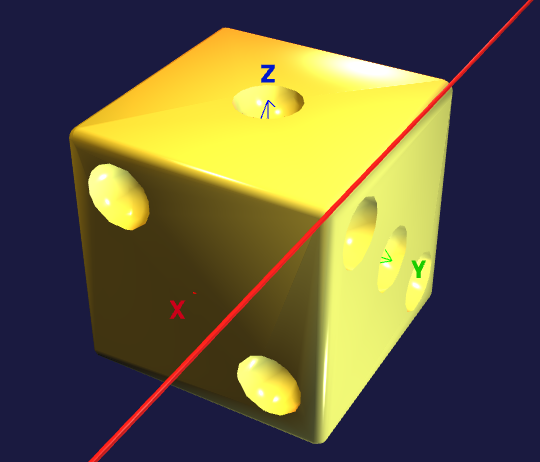
\includegraphics[width=0.6\textwidth]{\fig/lab3_es3_line.png}

Nell'immagine, la retta di cui parla l'esercizio \`e segnata in rosso

\end{frame}

\begin{frame}
\frametitle{Esercizio 3 - traccia di soluzione}
Non abbiamo una formula per rotazioni intorno ad un asse generico. Tuttavia,
in questo caso possiamo:
    \begin{enumerate}
        \item Traslare il dado di un vettore tale che il punto $P$ venga traslato sull'origine degli assi ($T_1$) \\
            $\Rightarrow$ In questa maniera, la retta rossa coincider\`a con l'asse X
        \item Applicare una rotazione intorno l'asse X ($R$)
        \item Traslare nuovamente il dado riportando il punto $P$ alla sua posizione iniziale ($T_2$)
    \end{enumerate}

    La trasformazione cercata sar\`a quindi la composizione delle tre trasformazioni, e la
    matrice che la rappresenta sar\`a $M= T_2 R T_1$.
\end{frame}

\begin{frame}
\frametitle{Esercizio 3 - i}
Voglio che il punto $P$ vada in $O$ origine degli assi: devo traslare del vettore
$\overrightarrow{PO}$.
\begin{displaymath}
    \overrightarrow{PO}
    = 
\begin{bmatrix}
        0 - P_x\\
        0 - P_y\\
        0 - P_z
\end{bmatrix}
    = 
\begin{bmatrix}
        - 1\\
        - 1\\
        - 1
\end{bmatrix}
\end{displaymath}
Quindi la matrice di traslazione in coordinate omogenee sar\`a:

\begin{displaymath}
T_1 = 
\begin{bmatrix}
        1 & 0 & 0 & -1\\
        0 & 1 & 0 & -1\\
        0 & 0 & 1 & -1\\
        0 & 0 & 0 & 1 
\end{bmatrix}
\end{displaymath}
\end{frame}

\begin{frame}
\frametitle{Esercizio 3 - ii}
La matrice R \`e una comune matrice di rotazione intorno all'asse X. \\
Ricordando che $cos(\nicefrac{\pi}{2}) = 0$ e $sin(\nicefrac{\pi}{2}) = 1$, abbiamo:
\begin{displaymath}
R
= 
\begin{bmatrix}
    1 & 0 & 0 & 0 \\
    0 &\mbox{cos}(\nicefrac{\pi}{2}) & -\mbox{sin}(\nicefrac{\pi}{2}) & 0\\
    0 &\mbox{sin}(\nicefrac{\pi}{2}) & \mbox{cos}(\nicefrac{\pi}{2})  & 0\\ 
    0 & 0 & 0 & 1
\end{bmatrix}
= 
\begin{bmatrix}
    1 & 0 & 0 & 0 \\
    0 & 0 & \shortminus 1 & 0\\
    0 & 1 & 0 & 0\\ 
    0 & 0 & 0 & 1
\end{bmatrix}
\end{displaymath}
\end{frame}

\begin{frame}
\frametitle{Esercizio 3 - iii}
Per l'ultimo step, voglio la traslazione che riporta lo spigolo del dado nella posizione
iniziale, quindi voglio andare dal punto $O$ in $P$. Scrivo il vettore $\overrightarrow{OP}$:
\begin{displaymath}
    \overrightarrow{OP}
    = 
\begin{bmatrix}
        P_x - 0\\
        P_y - 0\\
        P_z - 0
\end{bmatrix}
    = 
\begin{bmatrix}
        1\\
        1\\
        1
\end{bmatrix}
\end{displaymath}
Quindi la matrice di traslazione in coordinate omogenee sar\`a:

\begin{displaymath}
T_2 = 
\begin{bmatrix}
        1 & 0 & 0 & 1\\
        0 & 1 & 0 & 1\\
        0 & 0 & 1 & 1\\
        0 & 0 & 0 & 1 
\end{bmatrix}
\end{displaymath}
\end{frame}

\begin{frame}
\frametitle{Esercizio 3 - iv}
Componiamo ora le tre trasformazioni per ottenere il risultato richiesto. Come gi\`a detto, $M = T_2 R T_1$.
Dobbiamo moltiplicare 3 matrici, iniziamo moltiplicando le due pi\`u a destra;
    per comodit\`a chiamiamo questo risultato intermedio $M_1$:
\begin{displaymath}
M_1    
    =
    R T_1
    =
\begin{bmatrix}
    1 & 0 &  0 & 0 \\
    0 & 0 & -1 & 0\\
    0 & 1 &  0 & 0\\ 
    0 & 0 &  0 & 1
\end{bmatrix}
\begin{bmatrix}
        1 & 0 & 0 & -1 \\
        0 & 1 & 0 & -1 \\
        0 & 0 & 1 & -1 \\
        0 & 0 & 0 & 1 
\end{bmatrix}
\end{displaymath}

    \begin{displaymath}
   M_1 = 
\begin{bmatrix}
    1 & 0 &  0 & -1 \\
    0 & 0 & -1 &  1 \\
    0 & 1 &  0 & -1 \\ 
    0 & 0 &  0 &  1
\end{bmatrix}
\end{displaymath}
\end{frame}

\begin{frame}
\frametitle{Esercizio 3 - v}
Eseguiamo ora una ulteriore moltiplicazione matrice-matrice per completare il calcolo di $M$:
\begin{displaymath}
M    
    =
    T_2 R T_1
    =
    T_2 M_1
    =
\begin{bmatrix}
    1 & 0 &  0 & 1 \\
    0 & 1 &  0 & 1 \\
    0 & 0 &  1 & 1 \\ 
    0 & 0 &  0 & 1
\end{bmatrix}
\begin{bmatrix}
    1 & 0 &  0 & -1 \\
    0 & 0 & -1 &  1 \\
    0 & 1 &  0 & -1 \\ 
    0 & 0 &  0 &  1
\end{bmatrix}
\end{displaymath}

    \begin{displaymath}
   M = 
\begin{bmatrix}
    1 & 0 &  0 &  0 \\
    0 & 0 & -1 &  2 \\
    0 & 1 &  0 &  0 \\ 
    0 & 0 &  0 &  1
\end{bmatrix}
\end{displaymath}
\end{frame}

\begin{frame}
\frametitle{Esercizio 3 - vi}
    \vspace{-0.75cm}
\begin{center}
\begin{tikzpicture}
\node(img1){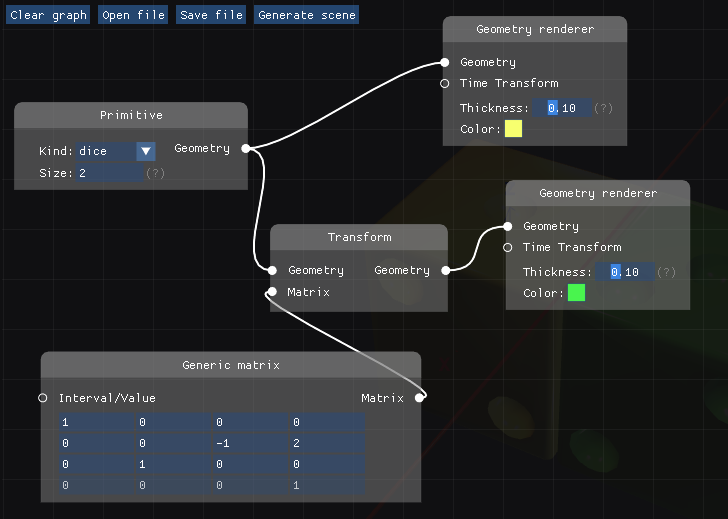
\includegraphics[width=0.8\textwidth]{\fig/lab3_es3_final_graph.png}};
\node(img2) at (img1.south east){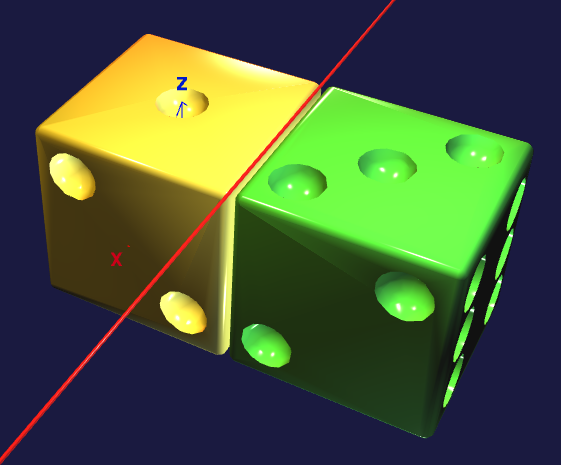
\includegraphics[width=0.4\textwidth]{\fig/lab3_es3_final_dice.png}};
\end{tikzpicture}
\end{center}
\end{frame}

\begin{frame}
\frametitle{Esercizio 3 - note}
    Nel calcolo di $M_1$ abbiamo composto \textbf{prima} una traslazione e \textbf{poi} una rotazione;
    abbiamo dovuto svolgere la moltiplicazione.
    
    Nel calcolo di $M$ invece la abbiamo composto \textbf{prima} una certa trasformazione e \textbf{poi} una traslazione.
    Quando l'ultima trasformazione applicata \`e una traslazione, abbiamo una scorciatoia! Siano date

\begin{displaymath}
    A = 
\begin{bmatrix}
    a_{11} & a_{12} & a_{13} & a_{14} \\
a_{21} & a_{22} & a_{23} & a_{24} \\
a_{31} & a_{32} & a_{33} & a_{34} \\
0      &    0   &  0     & 1 
\end{bmatrix}
    \quad
    T = 
\begin{bmatrix}
    1 & 0 & 0 & t_x \\
    0 & 1 & 0 & t_y \\
    0 & 0 & 1 & t_z \\
0      &    0   &  0     & 1 
\end{bmatrix}
\end{displaymath}
Allora
\begin{displaymath}
T A
    =  
\begin{bmatrix}
a_{11} & a_{12} & a_{13} & a_{14} + t_x\\
a_{21} & a_{22} & a_{23} & a_{24} + t_y\\
a_{31} & a_{32} & a_{33} & a_{34} + t_z\\
0      &    0   &  0     & 1 
\end{bmatrix}
\end{displaymath}

\end{frame}

\begin{frame}
\frametitle{Esercizio 3 - note}
Nel nostro caso specifico:
\begin{displaymath}
   M_1 = 
\begin{bmatrix}
    1 & 0 &  0 & \shortminus 1 \\
    0 & 0 & \shortminus 1 &  1 \\
    0 & 1 &  0 & \shortminus 1 \\ 
    0 & 0 &  0 &  1
\end{bmatrix}
\quad
T_2 = 
\begin{bmatrix}
        1 & 0 & 0 & 1\\
        0 & 1 & 0 & 1\\
        0 & 0 & 1 & 1\\
        0 & 0 & 0 & 1 
\end{bmatrix}
\end{displaymath}
\begin{displaymath}
M    
    =
    T_2 M_1
    =
\begin{bmatrix}
    1 & 0 &  0 & (\shortminus 1 + 1) \\
    0 & 0 & \shortminus 1 & (1 + 1) \\
    0 & 1 &  0 & (\shortminus 1 + 1) \\ 
    0 & 0 &  0 &  1
\end{bmatrix}
   = 
\begin{bmatrix}
    1 & 0 &  0 &  0 \\
    0 & 0 & \shortminus 1 &  2 \\
    0 & 1 &  0 &  0 \\ 
    0 & 0 &  0 &  1
\end{bmatrix}
\end{displaymath}

Sottolineiamo che questo \`e possibile \textbf{solo se la traslazione viene applicata dopo} l'altra generica trasformazione.
\end{frame}


\end{document}
